% Written by src/detection/final_figures.py; needs \usepackage{graphicx} and results/figures/ in \graphicspath.
\begin{figure*}[tb]
  \centering
  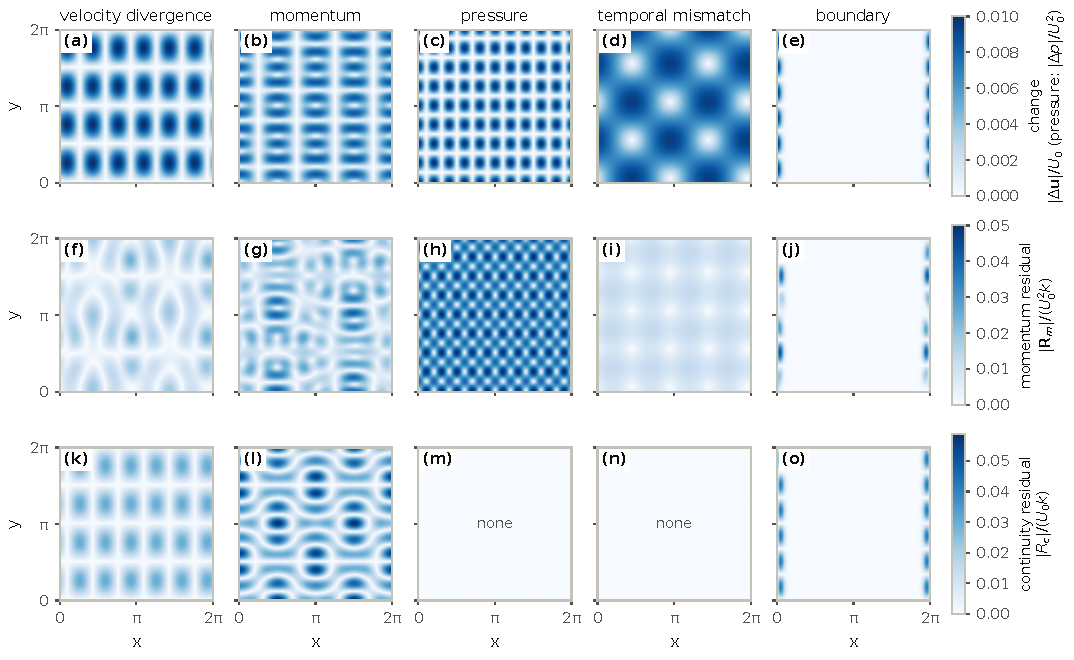
\includegraphics[width=\textwidth]{fig_damage_fields.pdf}
  \caption{What each synthetic damage does, at $\varepsilon = 0.01$, to the exact solution of case 34 ($k = 1$, $U_0 = 1.17$, Re $= 50.1$) at $t = 1$, half its time window, on a $128\times128$ grid of the periodic square ($x$ across, $y$ up). Top row: the change it makes, the velocity change $|\Delta\mathbf{u}|/U_0$, or for the pressure damage, which leaves the velocity alone, the pressure change $|\Delta p|/U_0^2$; middle row: the momentum residual it creates, $|\mathbf{R}_m|/(U_0^2 k)$; bottom row: its continuity residual, $|R_c|/(U_0 k)$. The residuals are scaled as in the scores, whose momentum and continuity terms are the mean squares of such maps over space and time. The exact solution has no residual, so every residual shown is the damage's own; a trained model, which differs from the exact solution by less than 1\%, gets nearly the same residual from the same damage. Each row has one colour scale. The pressure and temporal mismatch damages keep the flow divergence-free. The time shift reports the velocity at a later time but keeps the pressure of the original one; its momentum residual is that mismatch.}
  \label{fig:damage_fields}
\end{figure*}
